\documentclass[a4paper,11pt]{article}
\usepackage[english]{babel}
\usepackage[utf8]{inputenc}
\usepackage[T1]{fontenc}
\usepackage[a4paper,margin=1.5cm,top=1.2cm,bottom=1.2cm]{geometry}
\usepackage{graphicx}
\usepackage{amsmath}
\usepackage{booktabs}
<<<<<<< HEAD
=======
\usepackage{siunitx}
>>>>>>> c4b7d17 (supercipotes)
\usepackage{float}
\usepackage{microtype}
\usepackage{newtxtext,newtxmath}
\usepackage{setspace}
\usepackage{fancyhdr}
\usepackage{longtable}
\setstretch{1.15}

\pagestyle{fancy}
\fancyhf{}
\fancyfoot[C]{\thepage}
\renewcommand{\headrulewidth}{0pt}
\renewcommand{\footrulewidth}{0pt}
\setlength{\headheight}{14pt}
\setlength{\footskip}{14pt}

\begin{document}

\title{M33. Interferences in the Quincke Tube}
<<<<<<< HEAD
\author{Andrés Vinuesa Espinosa and José María Martínez Herrada}
=======
\author{Andrés Vinuesa Espinosa}
>>>>>>> c4b7d17 (supercipotes)
\maketitle

\begin{abstract}
This report investigates the phenomenon of acoustic interference using a Quincke tube. By measuring the transmitted sound intensity as a function of both frequency and path length difference, constructive and destructive interference patterns were identified. These observations were used to determine the speed of sound and the characteristic length of the apparatus. The experimental results for the speed of sound were compared with theoretical values calculated from the ambient temperature.
\end{abstract}

\section{Introduction and Objectives}

\subsection{Objectives}
\begin{itemize}
    \item Verify the occurrence of constructive and destructive interference in sound waves.
    \item Determine the speed of sound through the analysis of interference patterns.
    \item Calculate the characteristic length of the Quincke tube.
\end{itemize}

\subsection{Theoretical Background}
Interference occurs when two or more waves coincide in space and time. In a Quincke tube, a pressure wave from a source is split into two paths of lengths $a$ and $b$. These waves interfere at a receiver. The path difference is given by:
\begin{equation}
    b - a = 2\Delta d
\end{equation}
where $\Delta d$ is the displacement of the movable arm. The condition for constructive interference (maxima) and destructive interference (minima) is:
\begin{equation}
    \Delta d = n \frac{c}{4f}
\end{equation}
where $n$ is a relative ordinal, $c$ is the speed of sound, and $f$ is the frequency. When the paths are equal ($a=b$), resonance frequencies can occur according to:
\begin{equation}
    f_n = n \frac{c}{2a}
\end{equation}

\section{Materials and Methods}

\subsection{Experimental Setup}
<<<<<<< HEAD
The experimental apparatus used to study acoustic interference consists of the following components:
\begin{itemize}
    \item \textbf{Quincke Tube:} A hollow metallic tube split into two branches of lengths $a$ and $b$. Branch $a$ is fixed, while branch $b$ contains a movable arm that allows changing its length.
    \item \textbf{Sound Source:} A speaker placed at the input of the tube. It is connected to a digital function generator configured to emit a pure sinusoidal wave with a zero offset of \ensuremath{0.000\,\mathrm{V}} and an amplitude kept below \ensuremath{0.500\,\mathrm{V}} to prevent annoying noise in the laboratory.
    \item \textbf{Receiver System:} A microphone with an integrated preamplifier placed at the joint output of the tube. The microphone signal is sent to a digital oscilloscope and an AC voltmeter (with a full scale of \ensuremath{2\,\mathrm{V}}) to measure the amplitude of the interfering waves in terms of voltage.
\end{itemize}

\subsection{Experimental Procedure}
The laboratory work was divided into two separate procedures to analyze how changing either the frequency or the path length affects the interference:

\subsubsection{Part 1: Resonance and Standing Waves ($a = b$)}
First, the movable arm was adjusted so that both branches of the Quincke tube had the same length ($a = b$). The function generator was turned on at a starting frequency of \ensuremath{1300\,\mathrm{Hz}}. The frequency was then increased slowly by adjusting the main dial. By looking at the voltmeter and the oscilloscope screen, we identified the consecutive frequencies that produced audible maxima (resonance peaks) and minima. The values of these frequencies and their corresponding peak voltages were written down.

\subsubsection{Part 2: Interference at a Fixed Frequency}
For the second part of the practice, the frequency of the generator was fixed at $f = \ensuremath{1576\,\mathrm{Hz}}$, which was one of the highest voltage maxima observed in the first experiment. The movable arm of the tube was pushed in until it was only \ensuremath{0.5\,\mathrm{cm}} away from the top. We then moved the arm outwards in manual increments of \ensuremath{0.5\,\mathrm{cm}} using the metric scale of the tube until reaching the end of the rail. At each position, we recorded the displacement $\Delta d$ and the voltage reading from the voltmeter to map the alternating pattern of constructive and destructive interference.

\section{Results and Data Analysis}

\subsection{Experimental Data}
The direct measurements obtained during the laboratory session are presented below. Table \ref{tab:exp_a} displays the voltage recorded at various frequencies to identify the resonance modes (Experiment A). Table \ref{tab:exp_c} displays the voltage measured as a function of the movable arm's displacement $\Delta d$ at a constant frequency of $f = 1576\,\mathrm{Hz}$ (Experiment C). 

\begin{table}[H]
    \centering
    \caption{Voltage vs. Frequency (Experiment A)}
    \label{tab:exp_a}
    \begin{tabular}{r r r r}
        \toprule
        {Frequency $f$ (Hz)} & {Voltage $V$ (V)} & {$u_f$ (Hz)} & {$u_V$ (V)} \\
        \midrule
        1280 & 1.3  & 64  & 0.07 \\
        1380 & 6.9  & 69  & 0.35 \\
        1460 & 0.9  & 73  & 0.05 \\
        1576 & 10.7 & 79  & 0.54 \\
        1660 & 4.1  & 83  & 0.21 \\
        1710 & 2.7  & 86  & 0.14 \\
        1810 & 1.7  & 91  & 0.09 \\
        1890 & 1.4  & 95  & 0.07 \\
        2000 & 1.0  & 100 & 0.05 \\
        2070 & 4.4  & 104 & 0.22 \\
        2120 & 1.3  & 106 & 0.07 \\
        2190 & 2.1  & 110 & 0.11 \\
        \bottomrule
    \end{tabular}
\end{table}

\begin{table}[H]
    \centering
    \caption{Voltage vs. Displacement at $f = 1576\,\mathrm{Hz}$ (Experiment C) --- Extracted Extrema}\label{tab:exp_c}
    \begin{tabular}{lc r r}
        \toprule
        Extrema Type & Order ($n$) & {Displacement $\Delta d$ (m)} & {Voltage $V$ (V)} \\
        \midrule
        Minimum & 1 & 0.045 & 0.5 \\
        Maximum & 1 & 0.078 & 2.6 \\
        Minimum & 2 & 0.103 & 0.4 \\
        Maximum & 2 & 0.110 & 14.3 \\
        Minimum & 3 & 0.185 & 0.4 \\
        Maximum & 3 & 0.230 & 14.1 \\
        Minimum & 4 & 0.245 & 0.8 \\
        Maximum & 4 & 0.310 & 10.6 \\
        \bottomrule
    \end{tabular}
\end{table}

\subsubsection*{Oscilloscope Captures}
Figure \ref{fig:oscilloscope} shows the raw signals observed on the oscilloscope for a state of constructive interference (maximum amplitude) and destructive interference (minimum amplitude).

\begin{figure}[H]
    \centering
     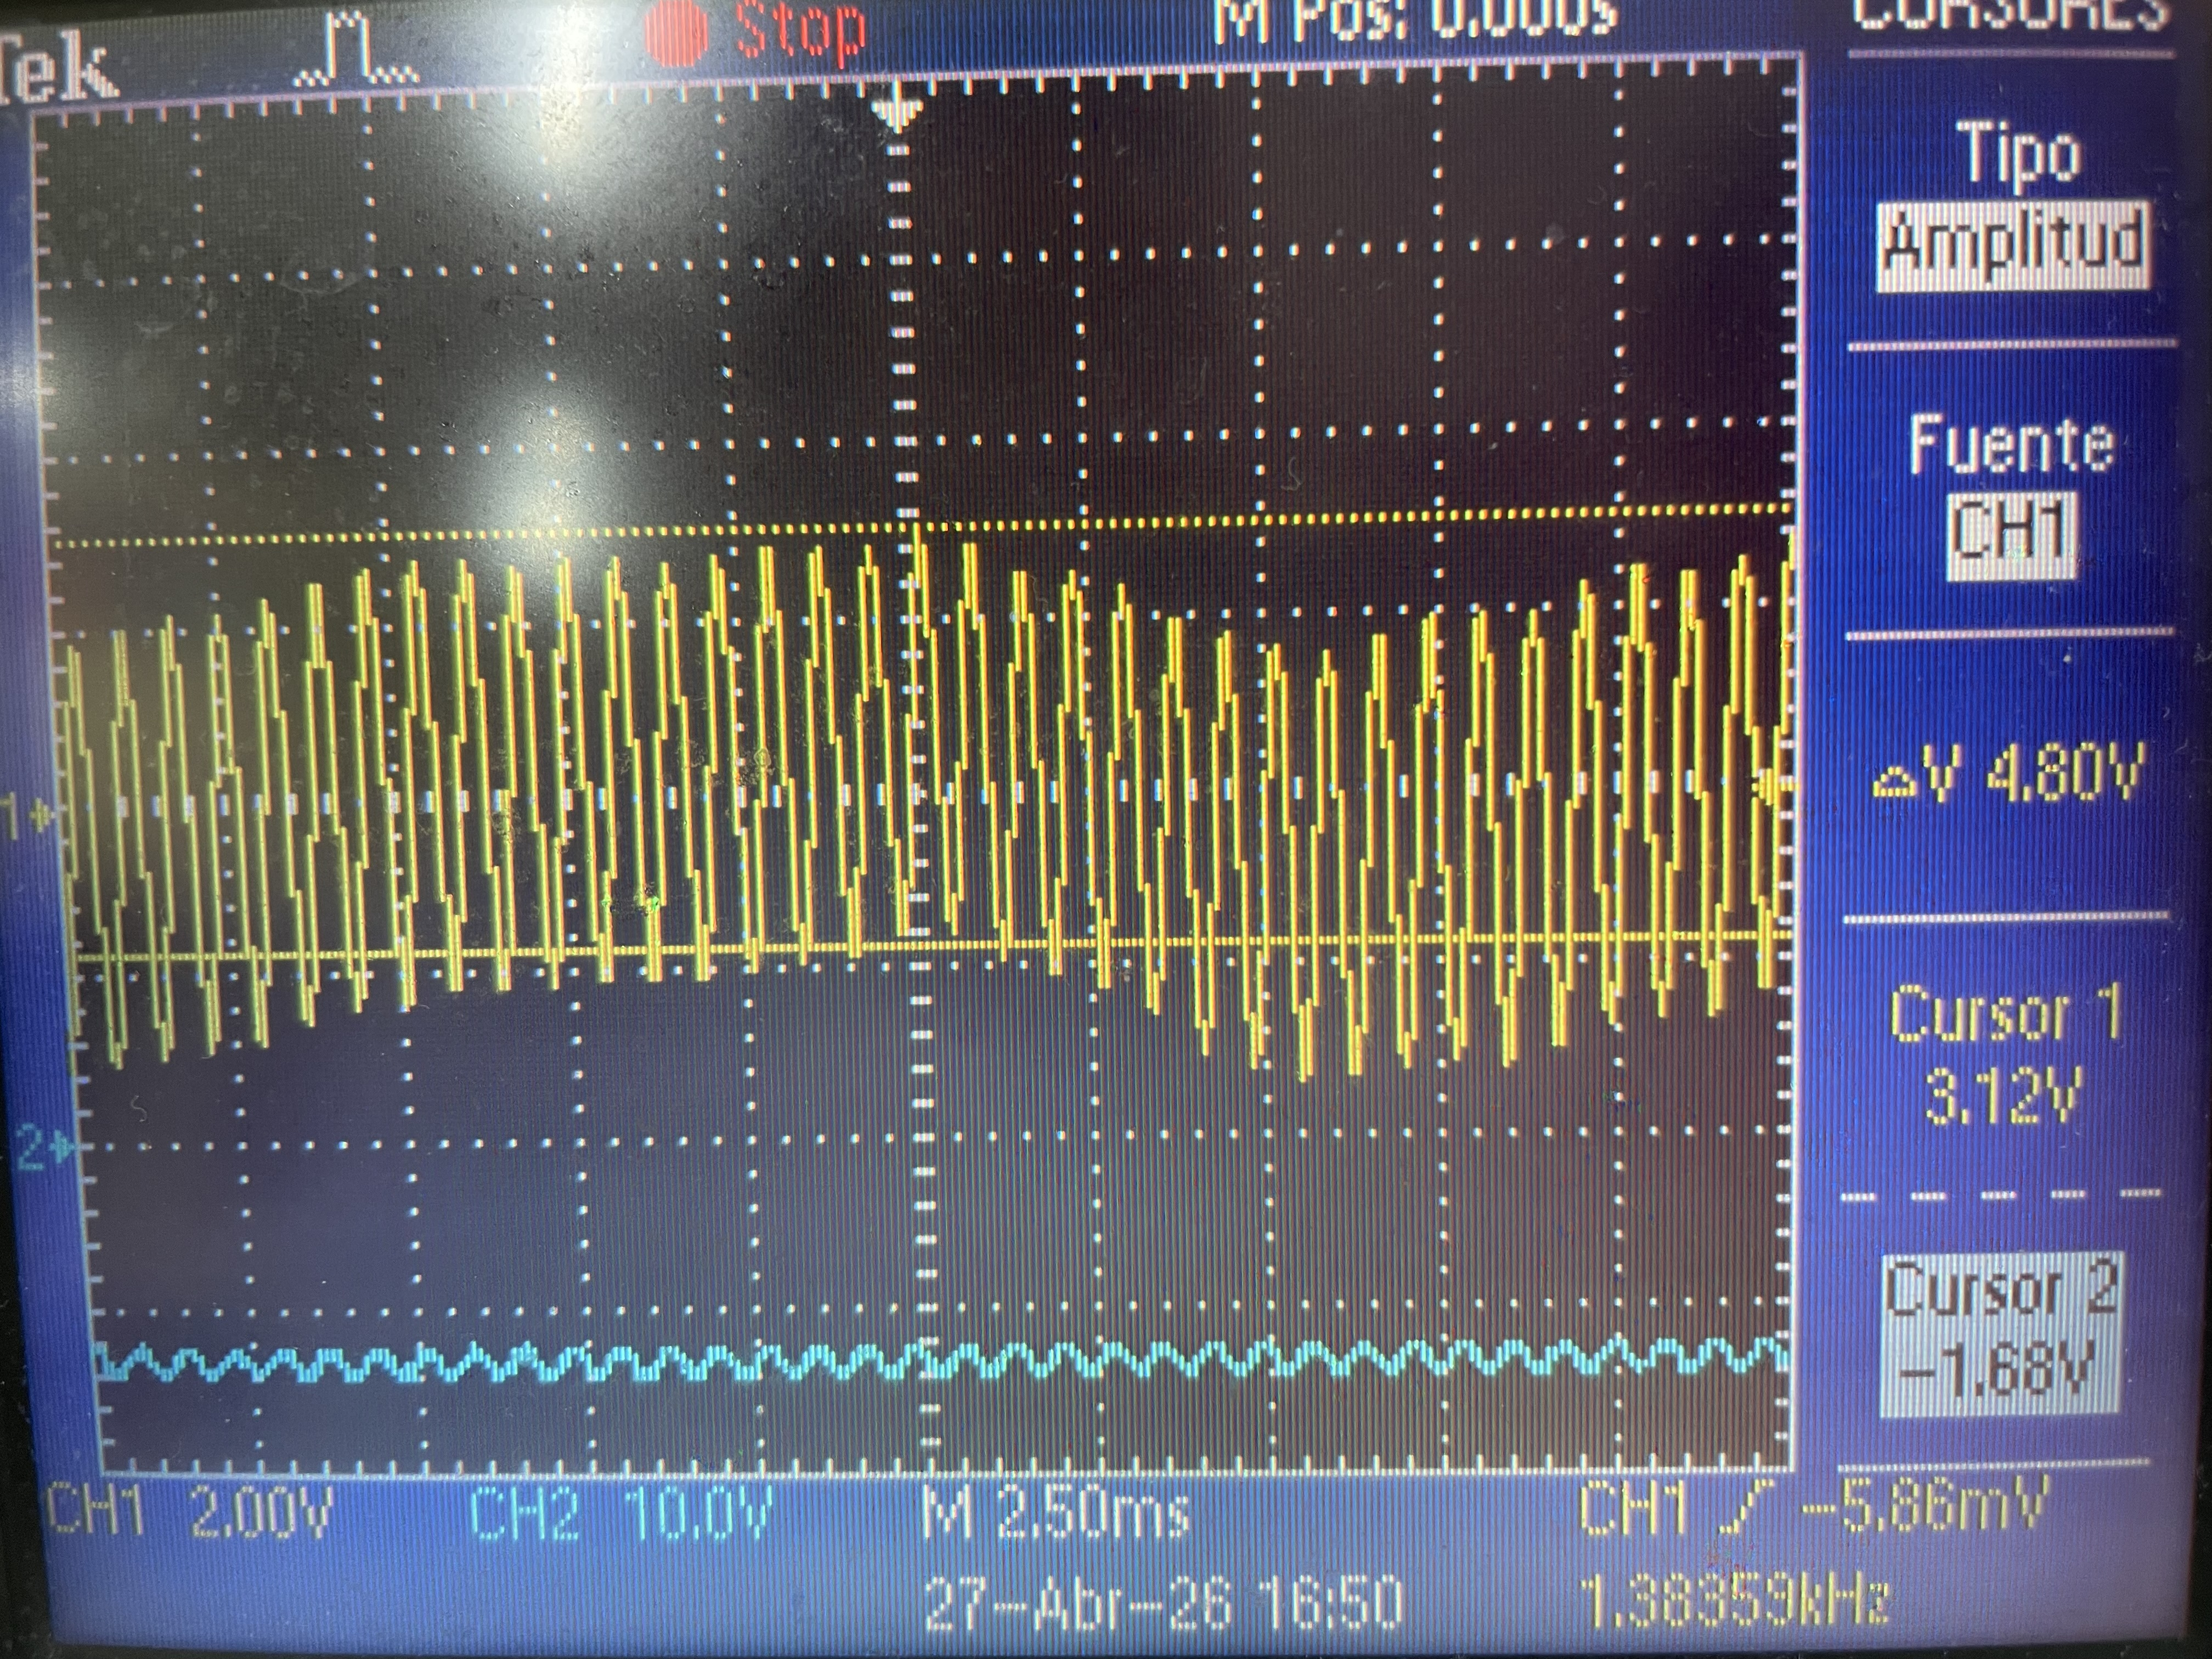
\includegraphics[width=0.45\textwidth]{IMG_6412.jpeg}
     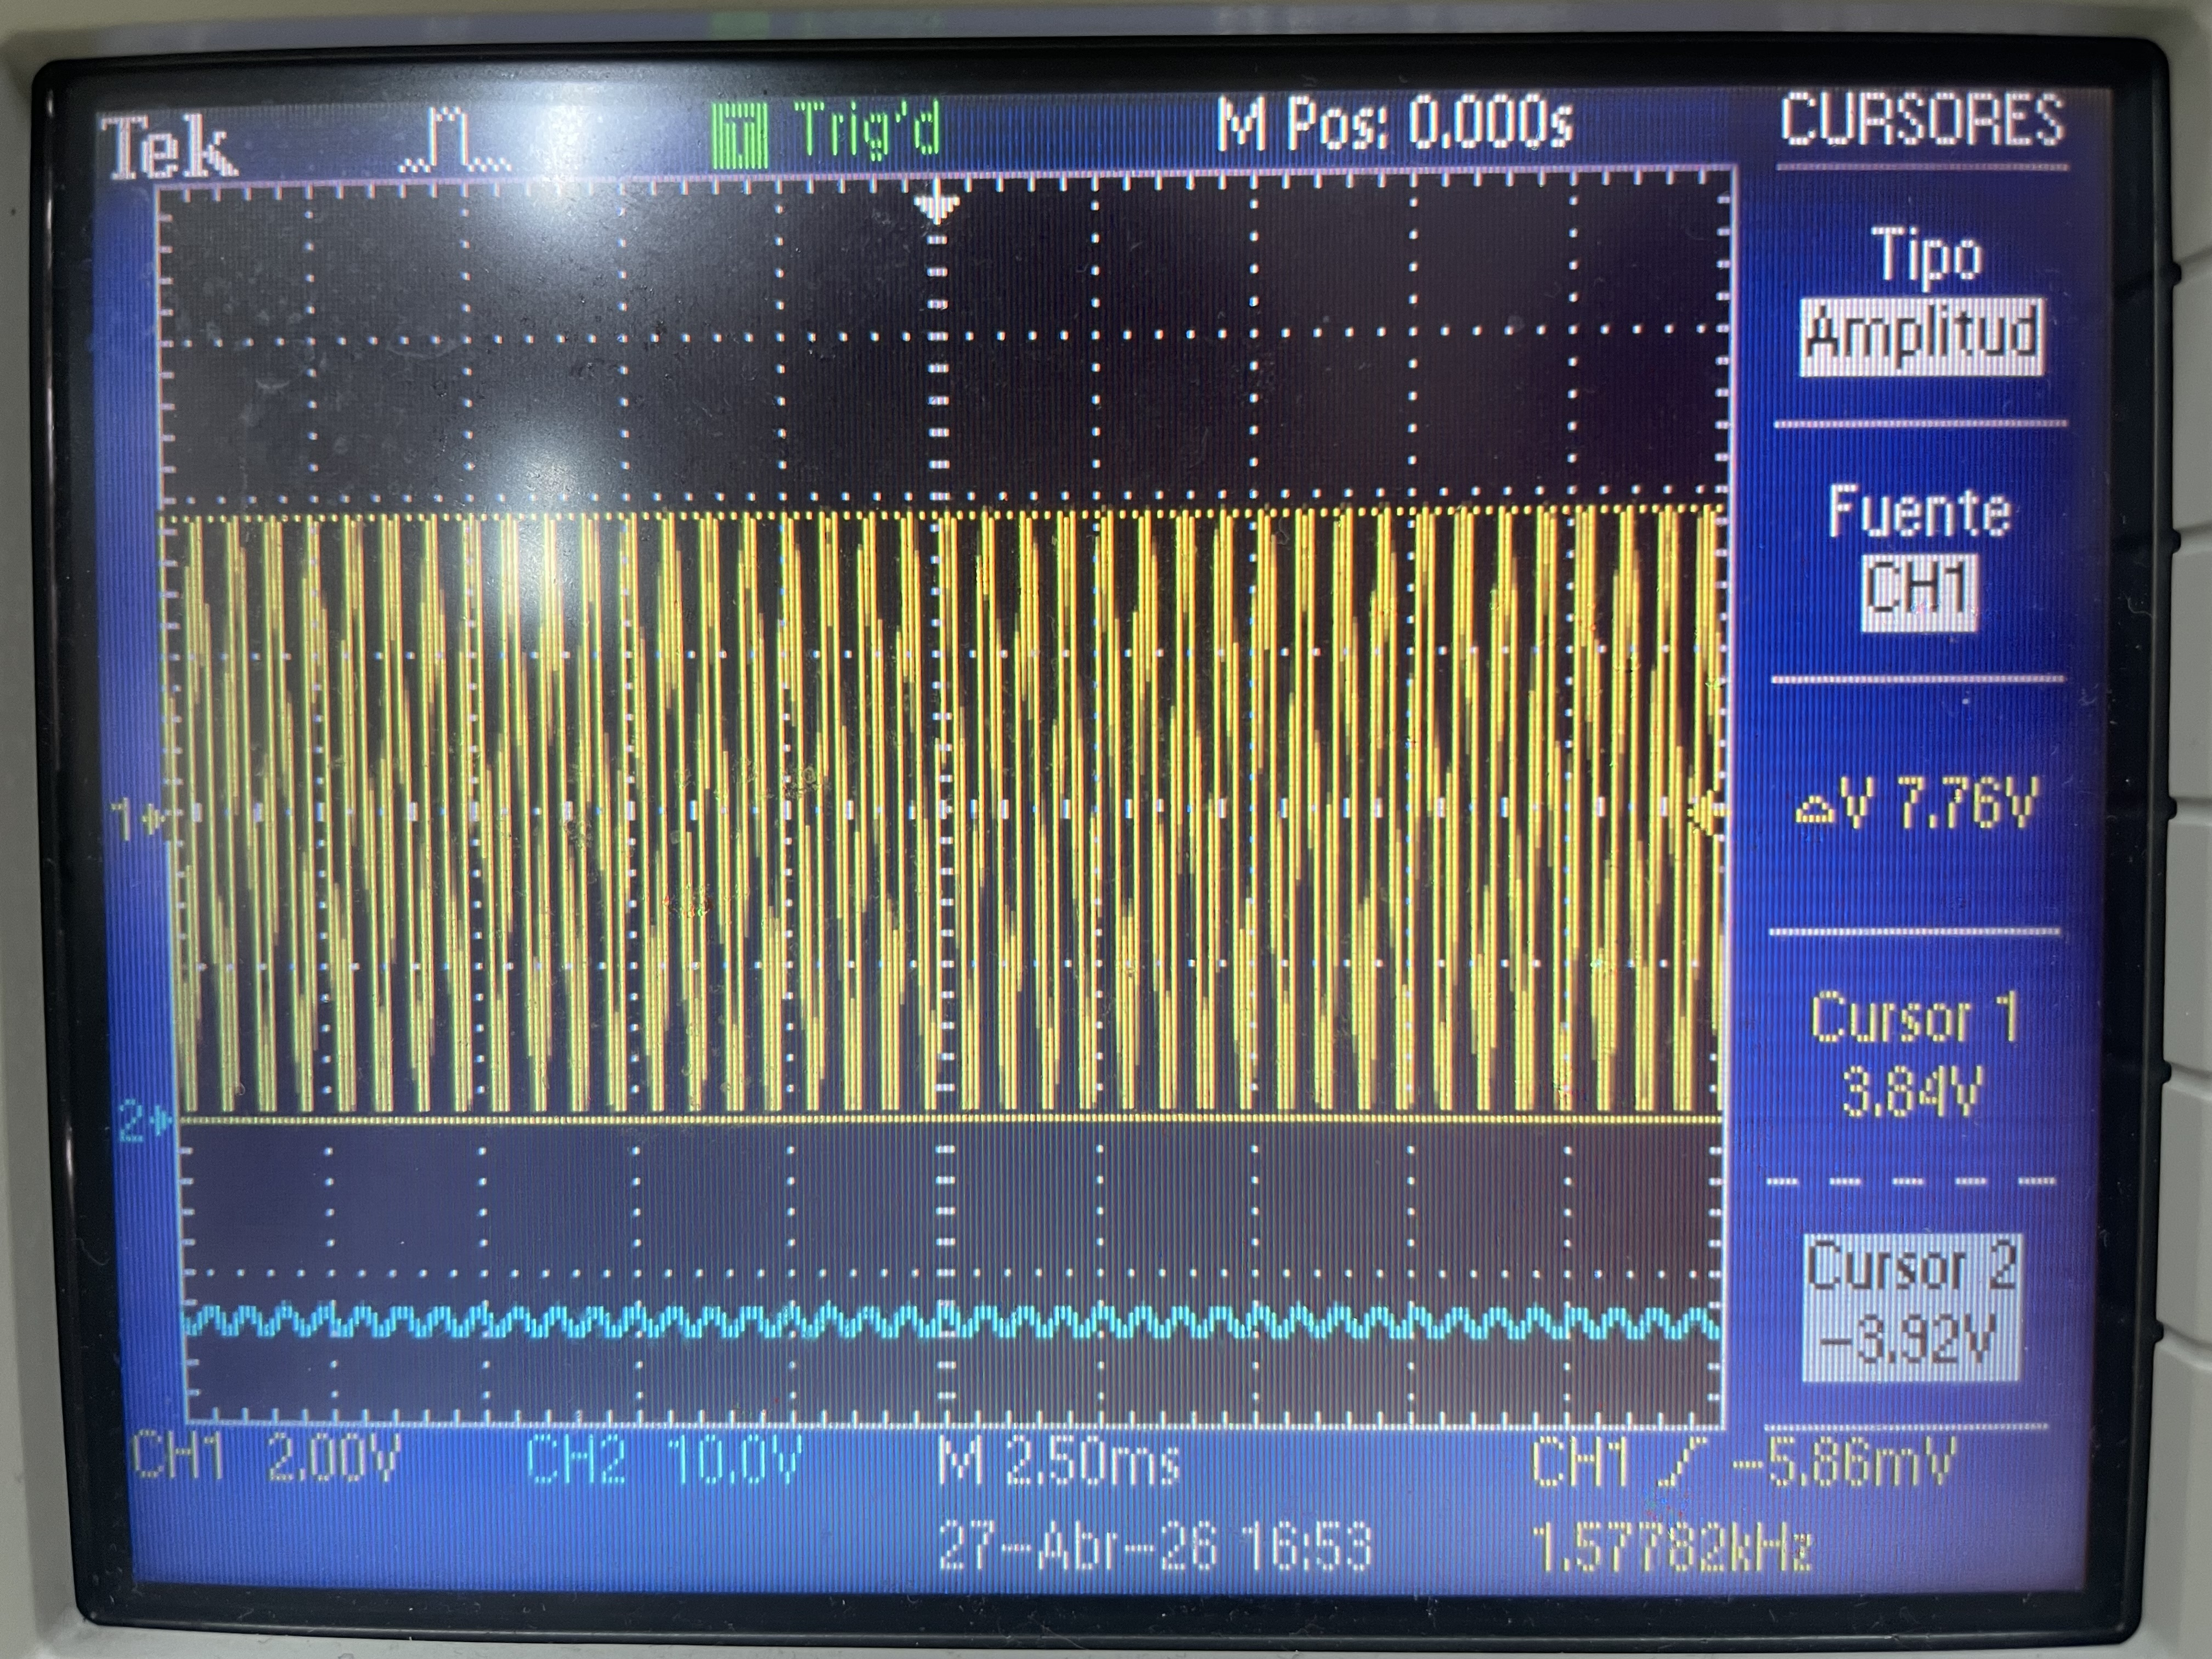
\includegraphics[width=0.45\textwidth]{IMG_6413.jpeg}
     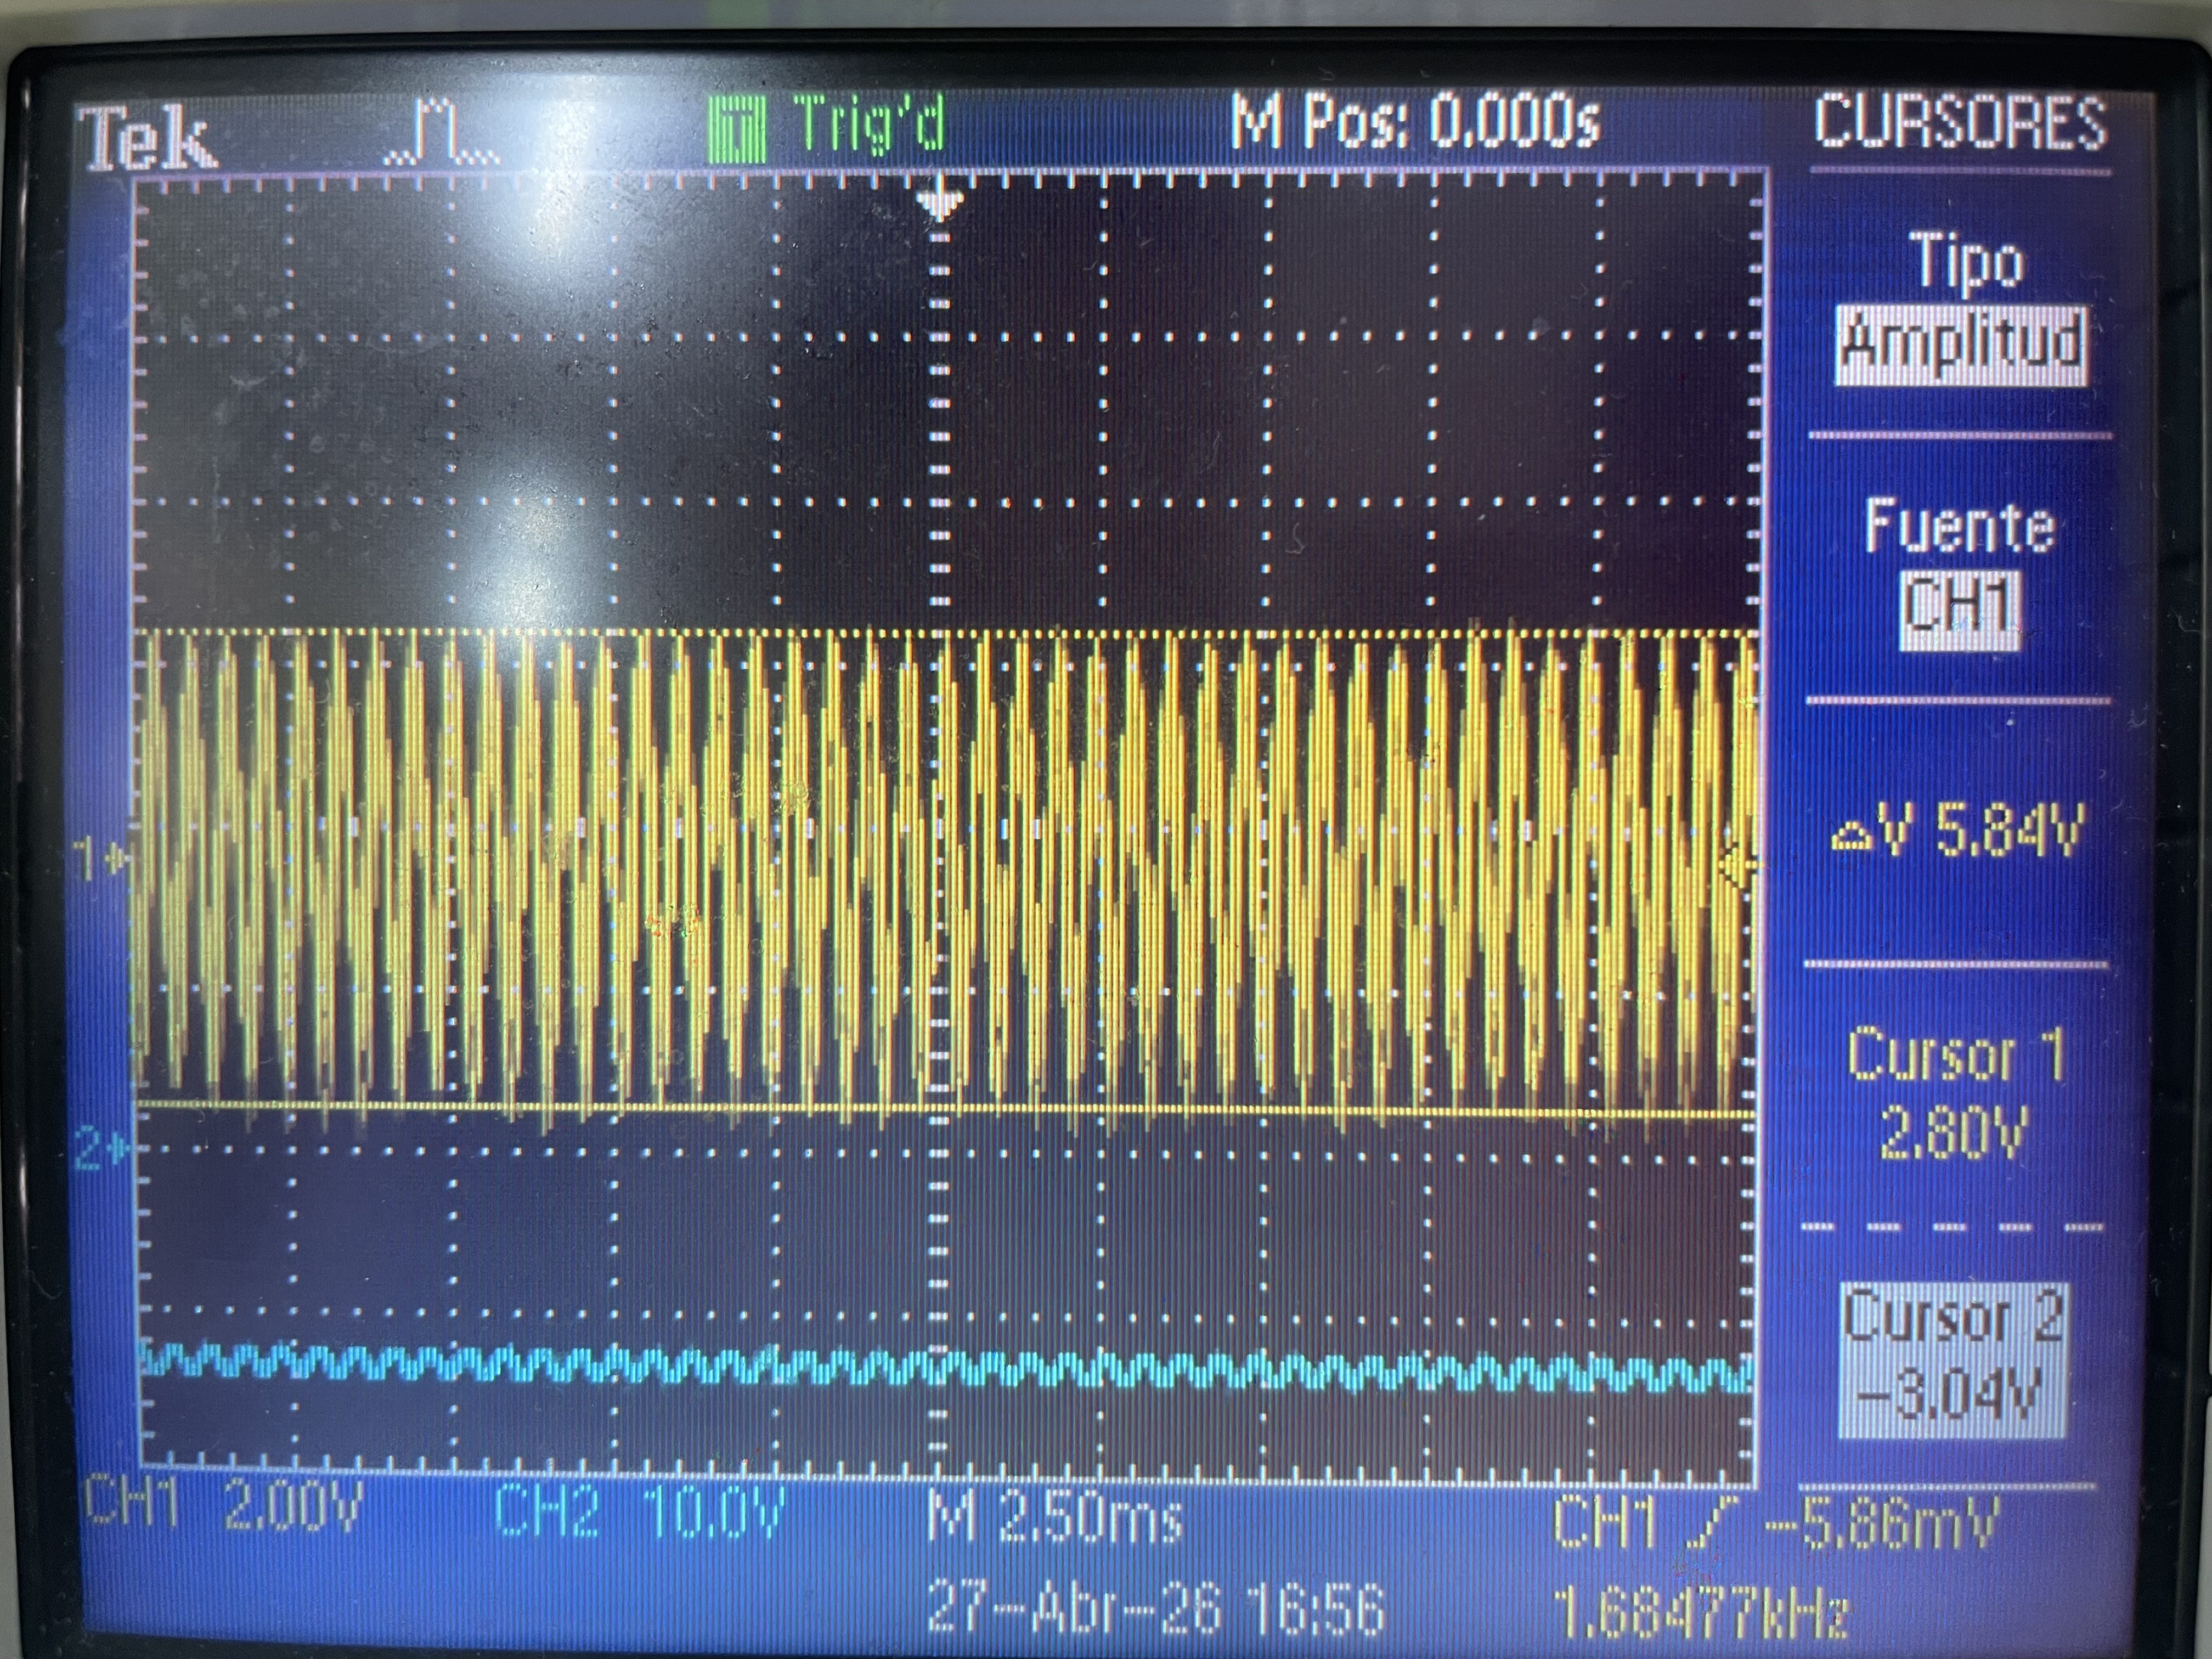
\includegraphics[width=0.45\textwidth]{IMG_6414.jpeg}
     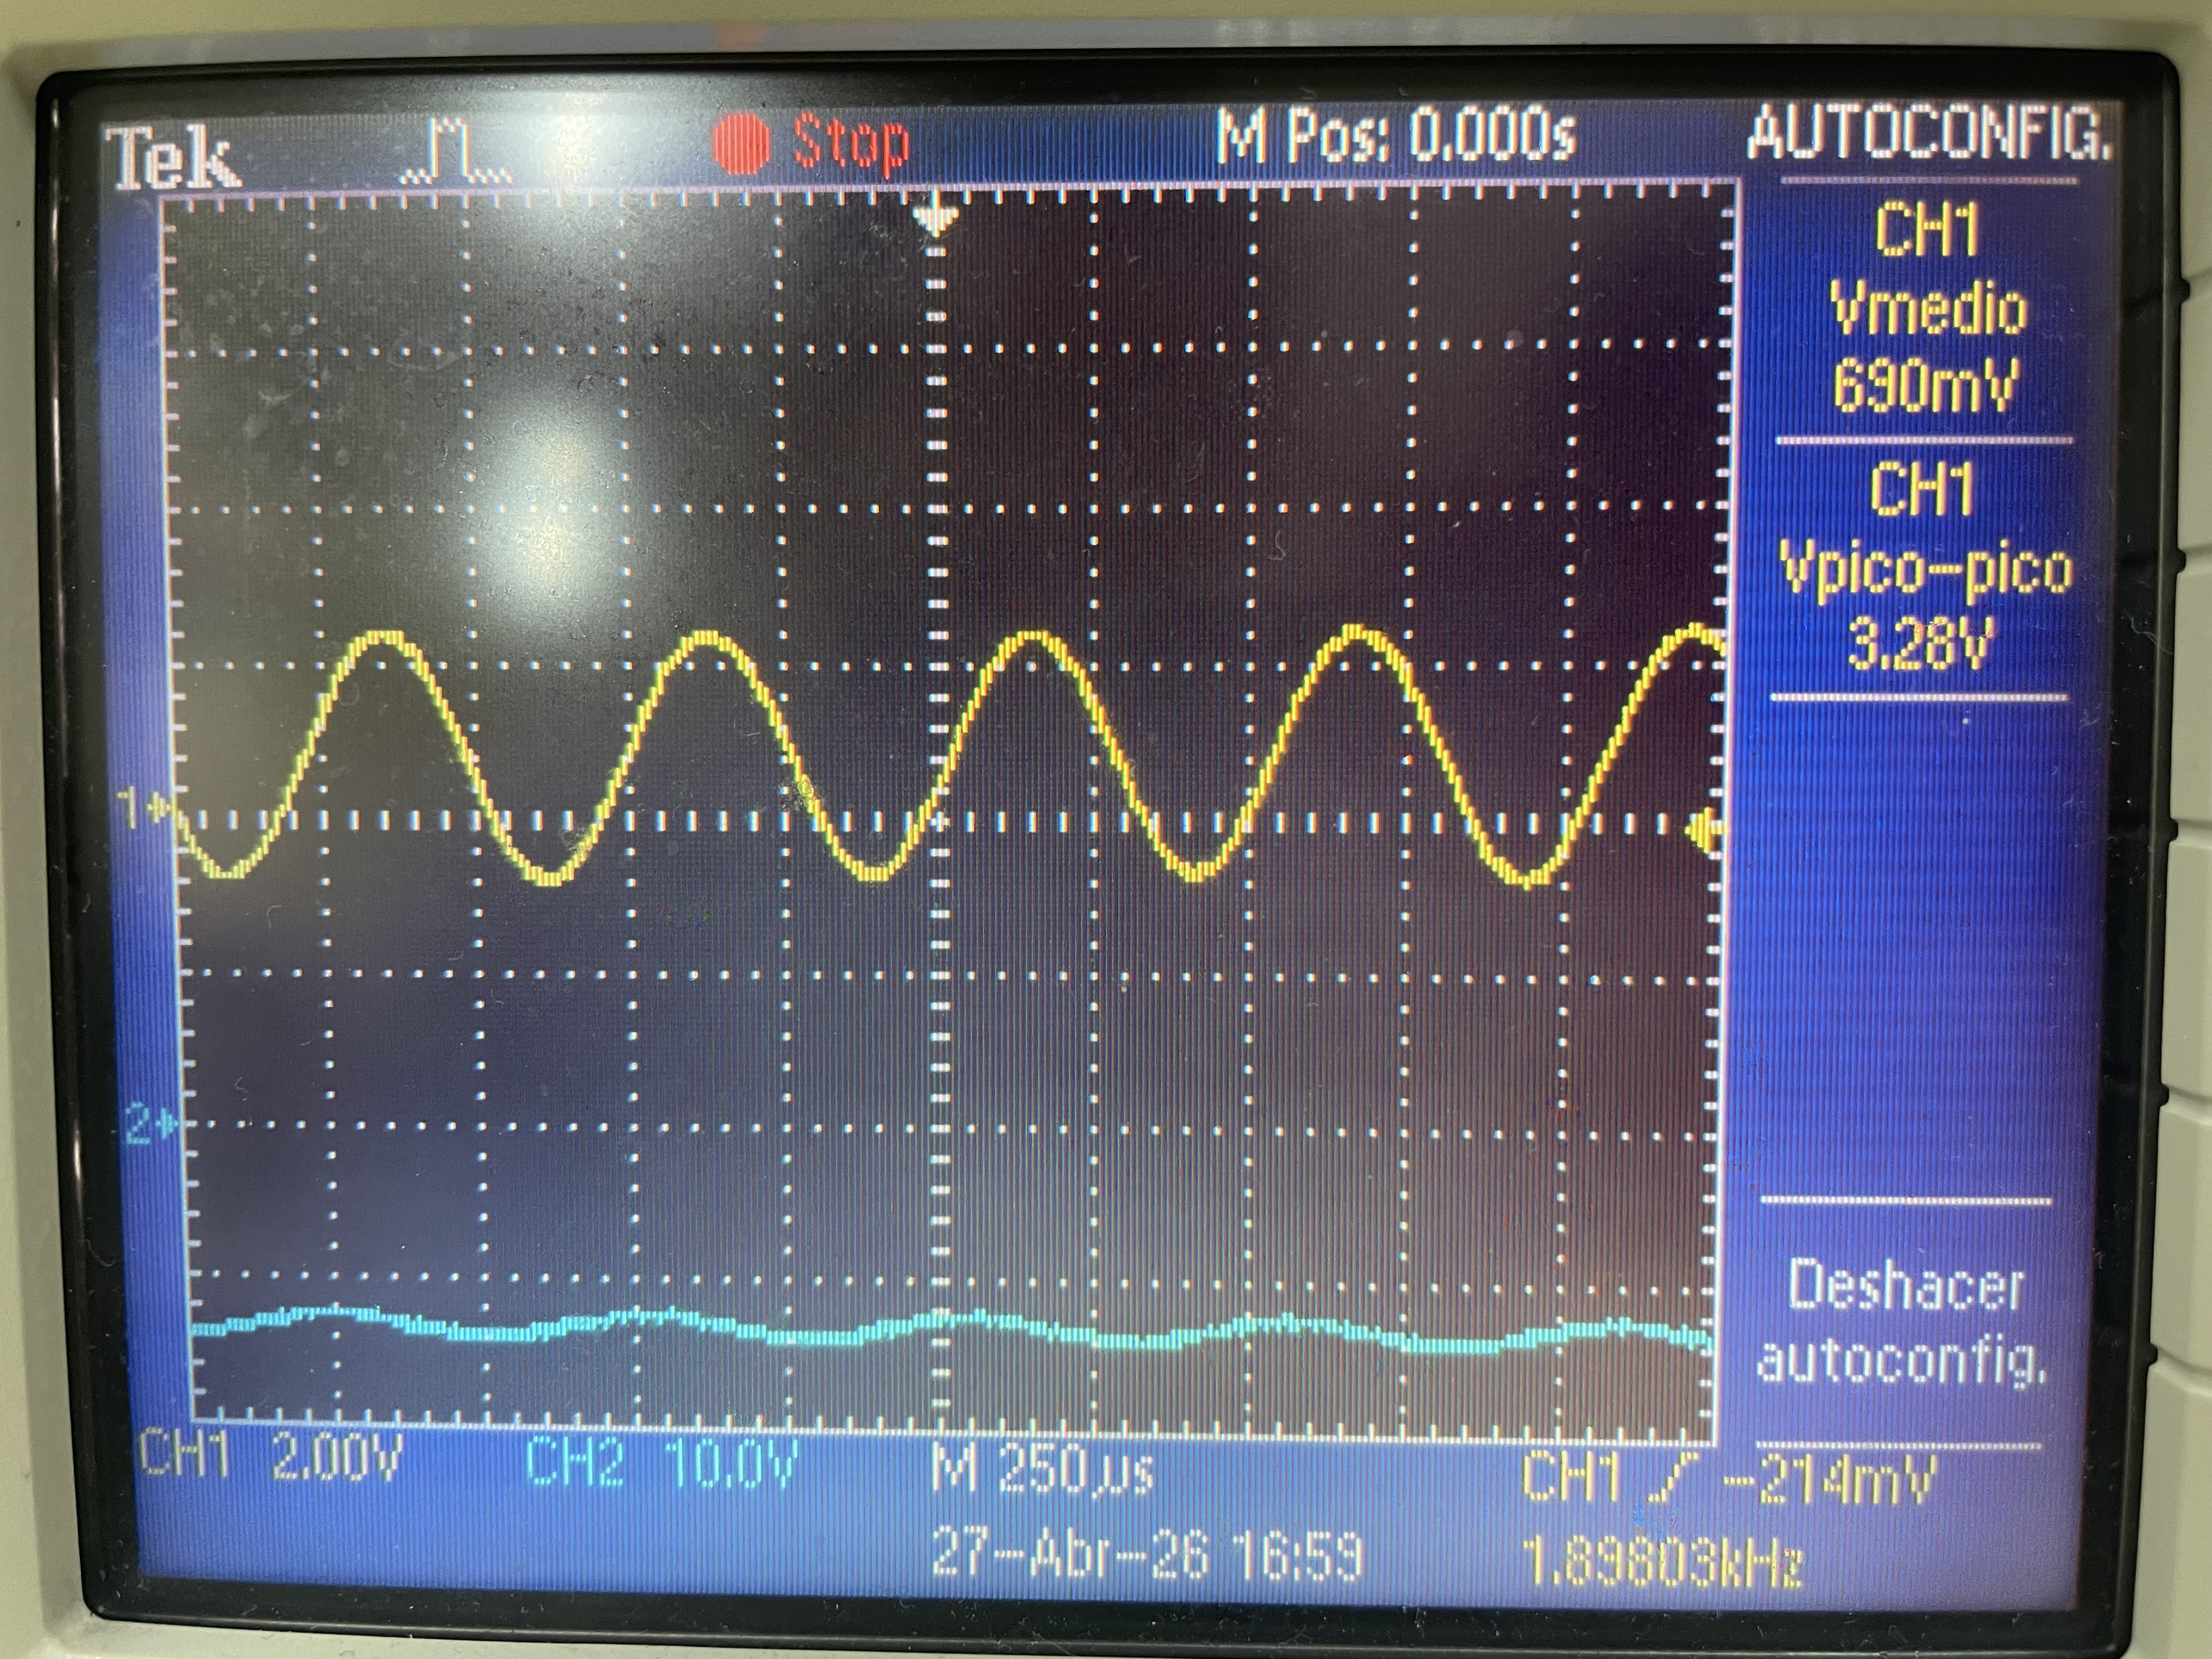
\includegraphics[width=0.45\textwidth]{IMG_6415.jpeg}
    \caption{Oscilloscope captures showing constructive (left) and destructive (right) interference.}
    \label{fig:oscilloscope}
\end{figure}

=======
The setup includes a Quincke tube with a movable arm, a speaker as a sound source connected to a function generator, and a microphone connected to a voltmeter or oscilloscope.

\subsection{Data Acquisition and Analysis}
Two main experiments were performed:
\begin{enumerate}
    \item \textbf{Experiment A/B}: Frequencies corresponding to maxima and minima were identified for a fixed tube configuration ($a \approx b$).
    \item \textbf{Experiment C}: The sound amplitude (voltage) was recorded as a function of the arm displacement $\Delta d$ for a fixed frequency $f = 1576$ Hz.
\end{enumerate}
The speed of sound $c$ was determined by fitting the positions of maxima and minima in Experiment C to the linear relation $\Delta d(n)$.

\section{Results and Data Analysis}

>>>>>>> c4b7d17 (supercipotes)
\subsection{Voltage vs Frequency}
The experimental results for the transmitted sound intensity as a function of frequency are displayed in Figure \ref{fig:v_vs_f}.

\begin{figure}[H]
    \centering
    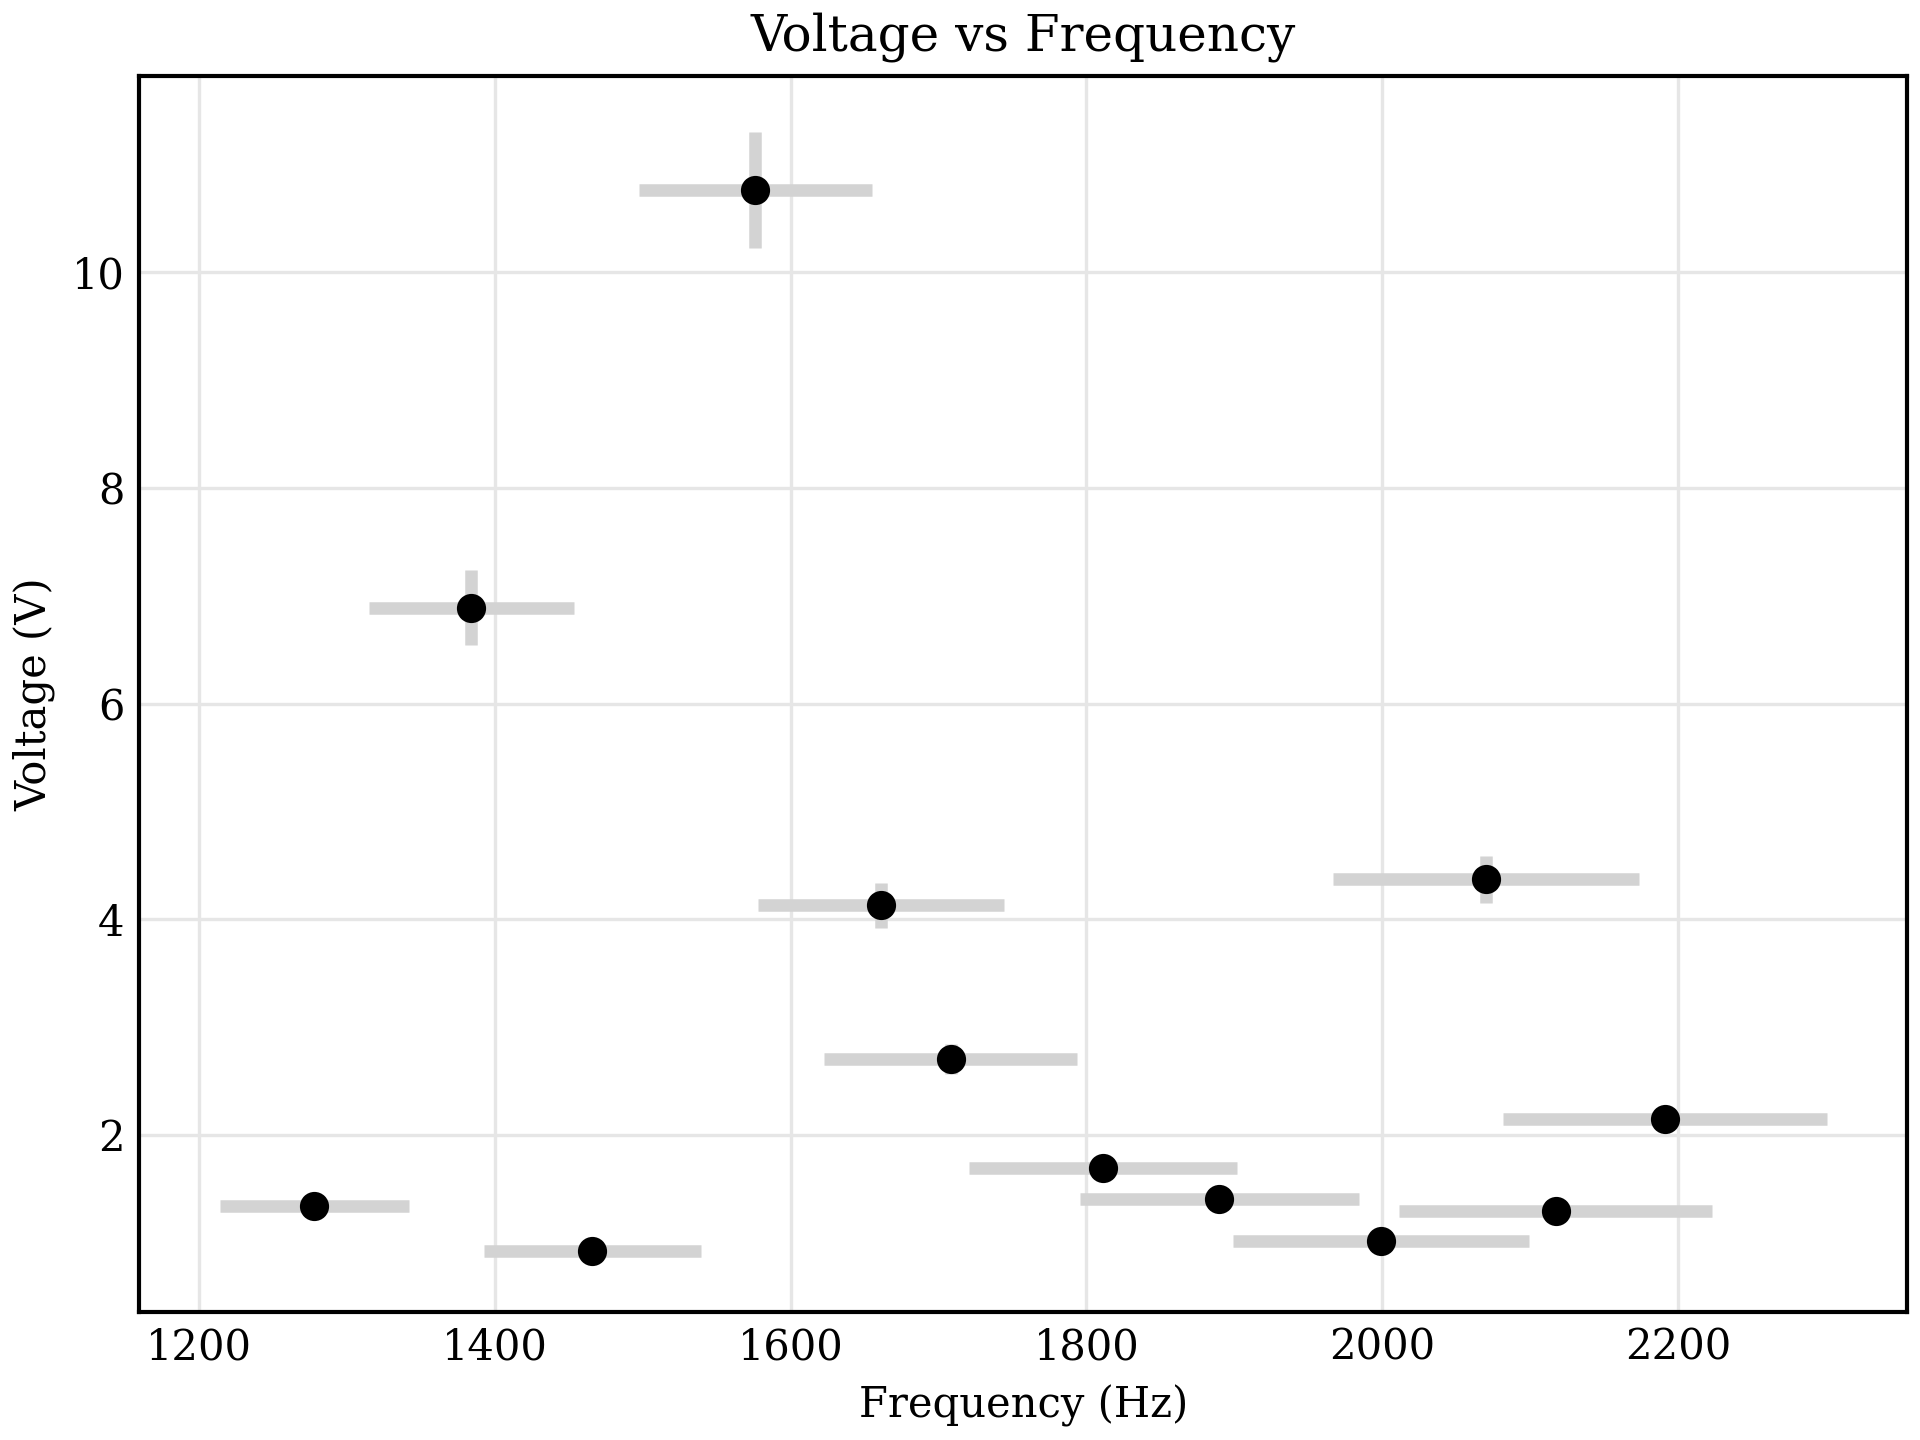
\includegraphics[width=0.8\textwidth]{m33_voltaje_vs_frecuencia.png}
    \caption{Sound amplitude (Voltage) as a function of source frequency.}
    \label{fig:v_vs_f}
\end{figure}

\subsection{Voltage vs Distance}
For a fixed frequency $f = 1576$ Hz, the voltage was measured as the arm displacement $\Delta d$ was varied. The resulting interference pattern is shown in Figure \ref{fig:v_vs_d_plot}.

\begin{figure}[H]
    \centering
    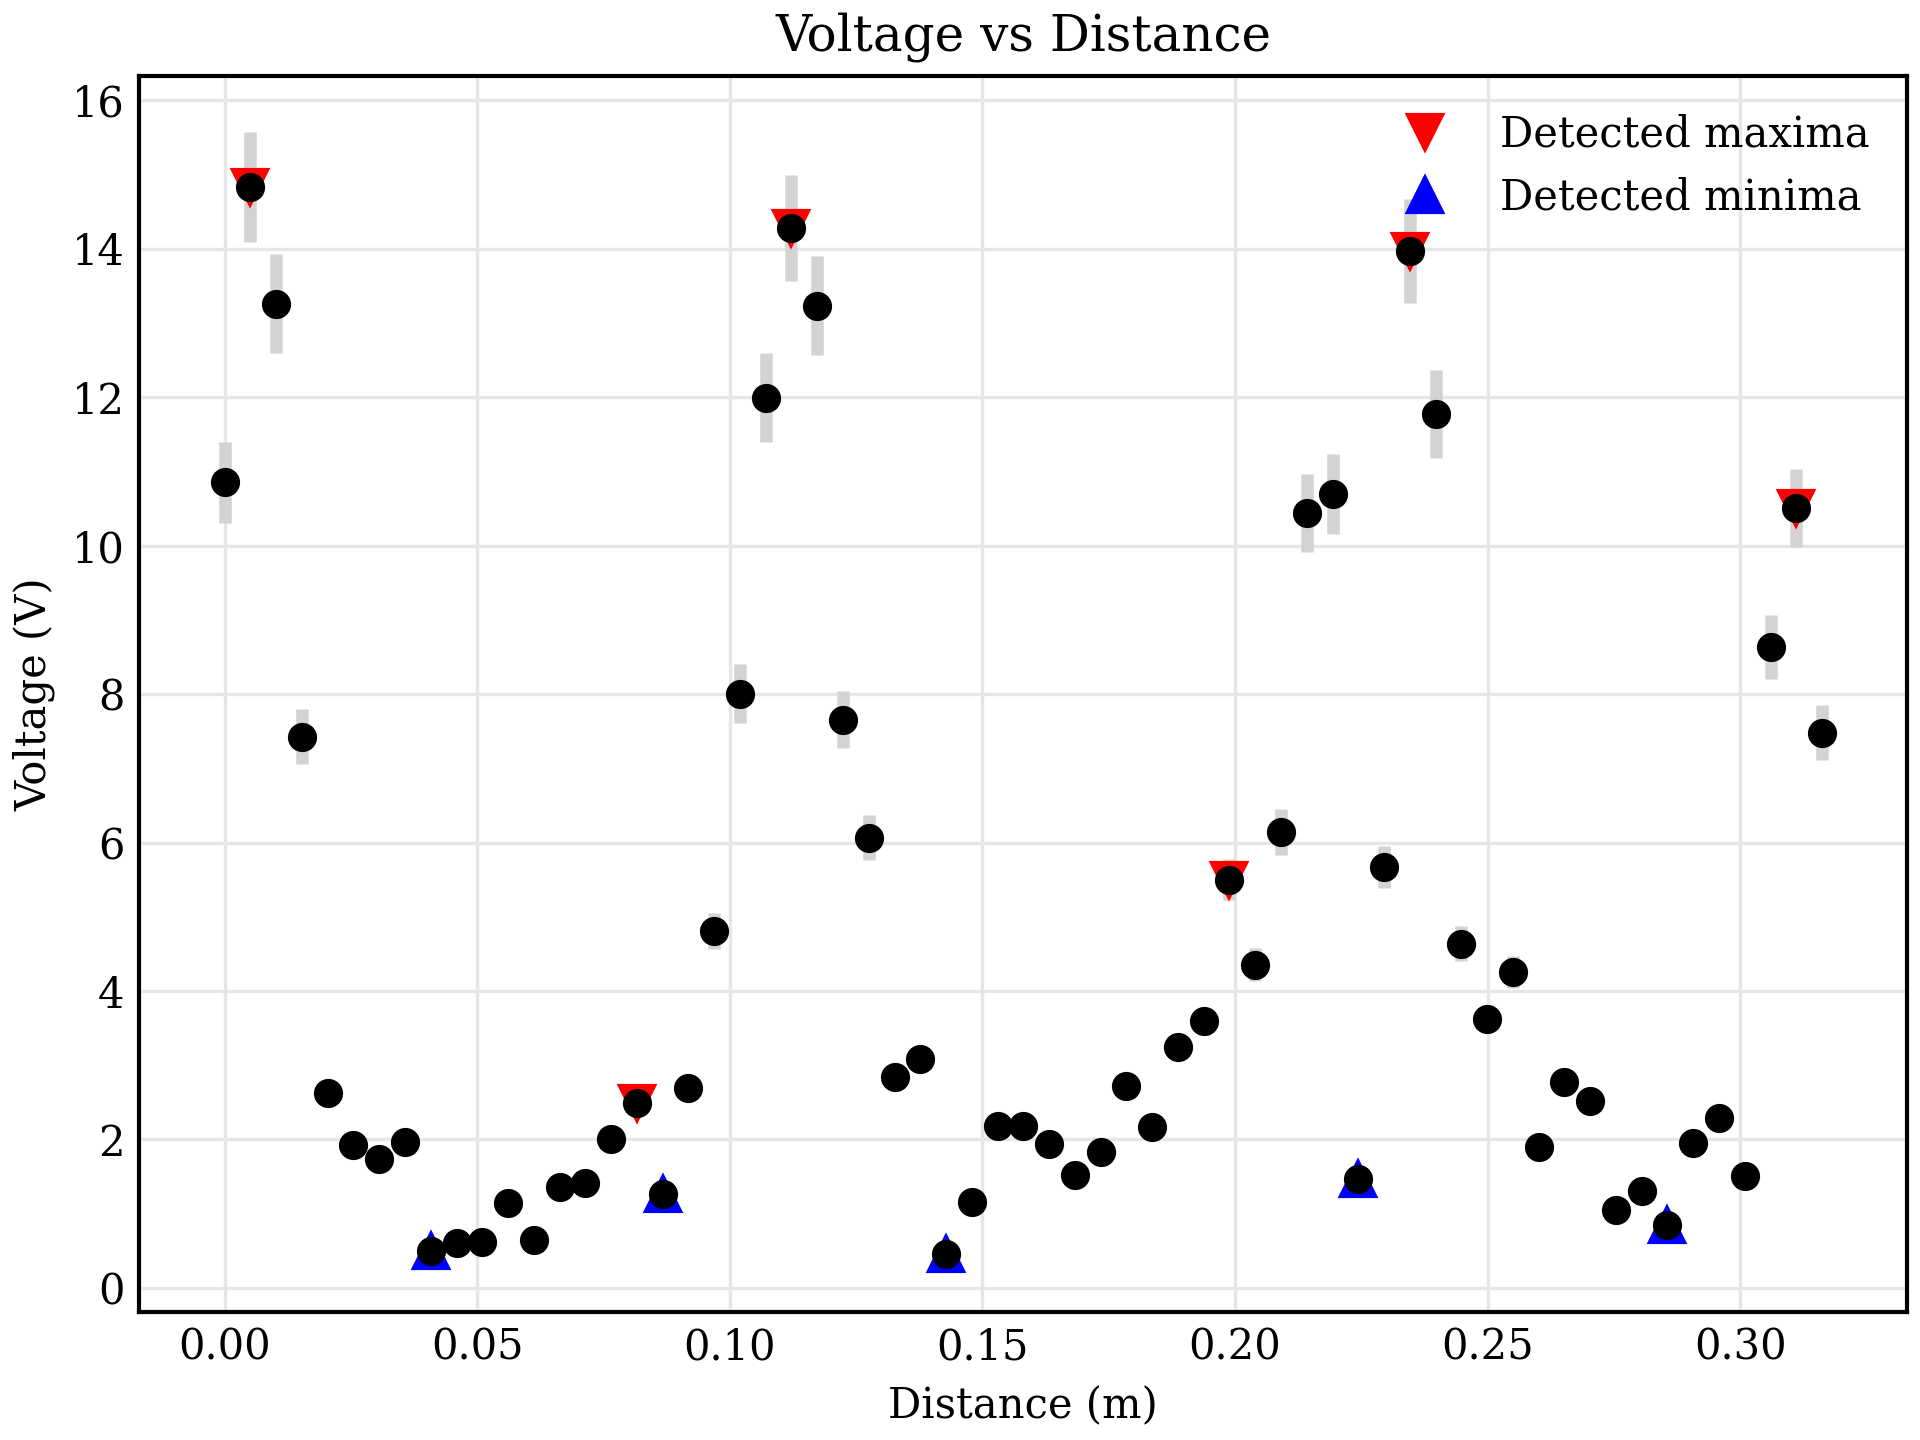
\includegraphics[width=0.8\textwidth]{m33_voltaje_vs_distancia.png}
    \caption{Sound amplitude (Voltage) as a function of movable arm displacement $\Delta d$.}
    \label{fig:v_vs_d_plot}
\end{figure}

\subsection{Determination of Sound Speed}
The detected peaks (maxima) and troughs (minima) from Experiment C were used to perform a linear fit of $\Delta d$ vs $n$.

\begin{figure}[H]
    \centering
    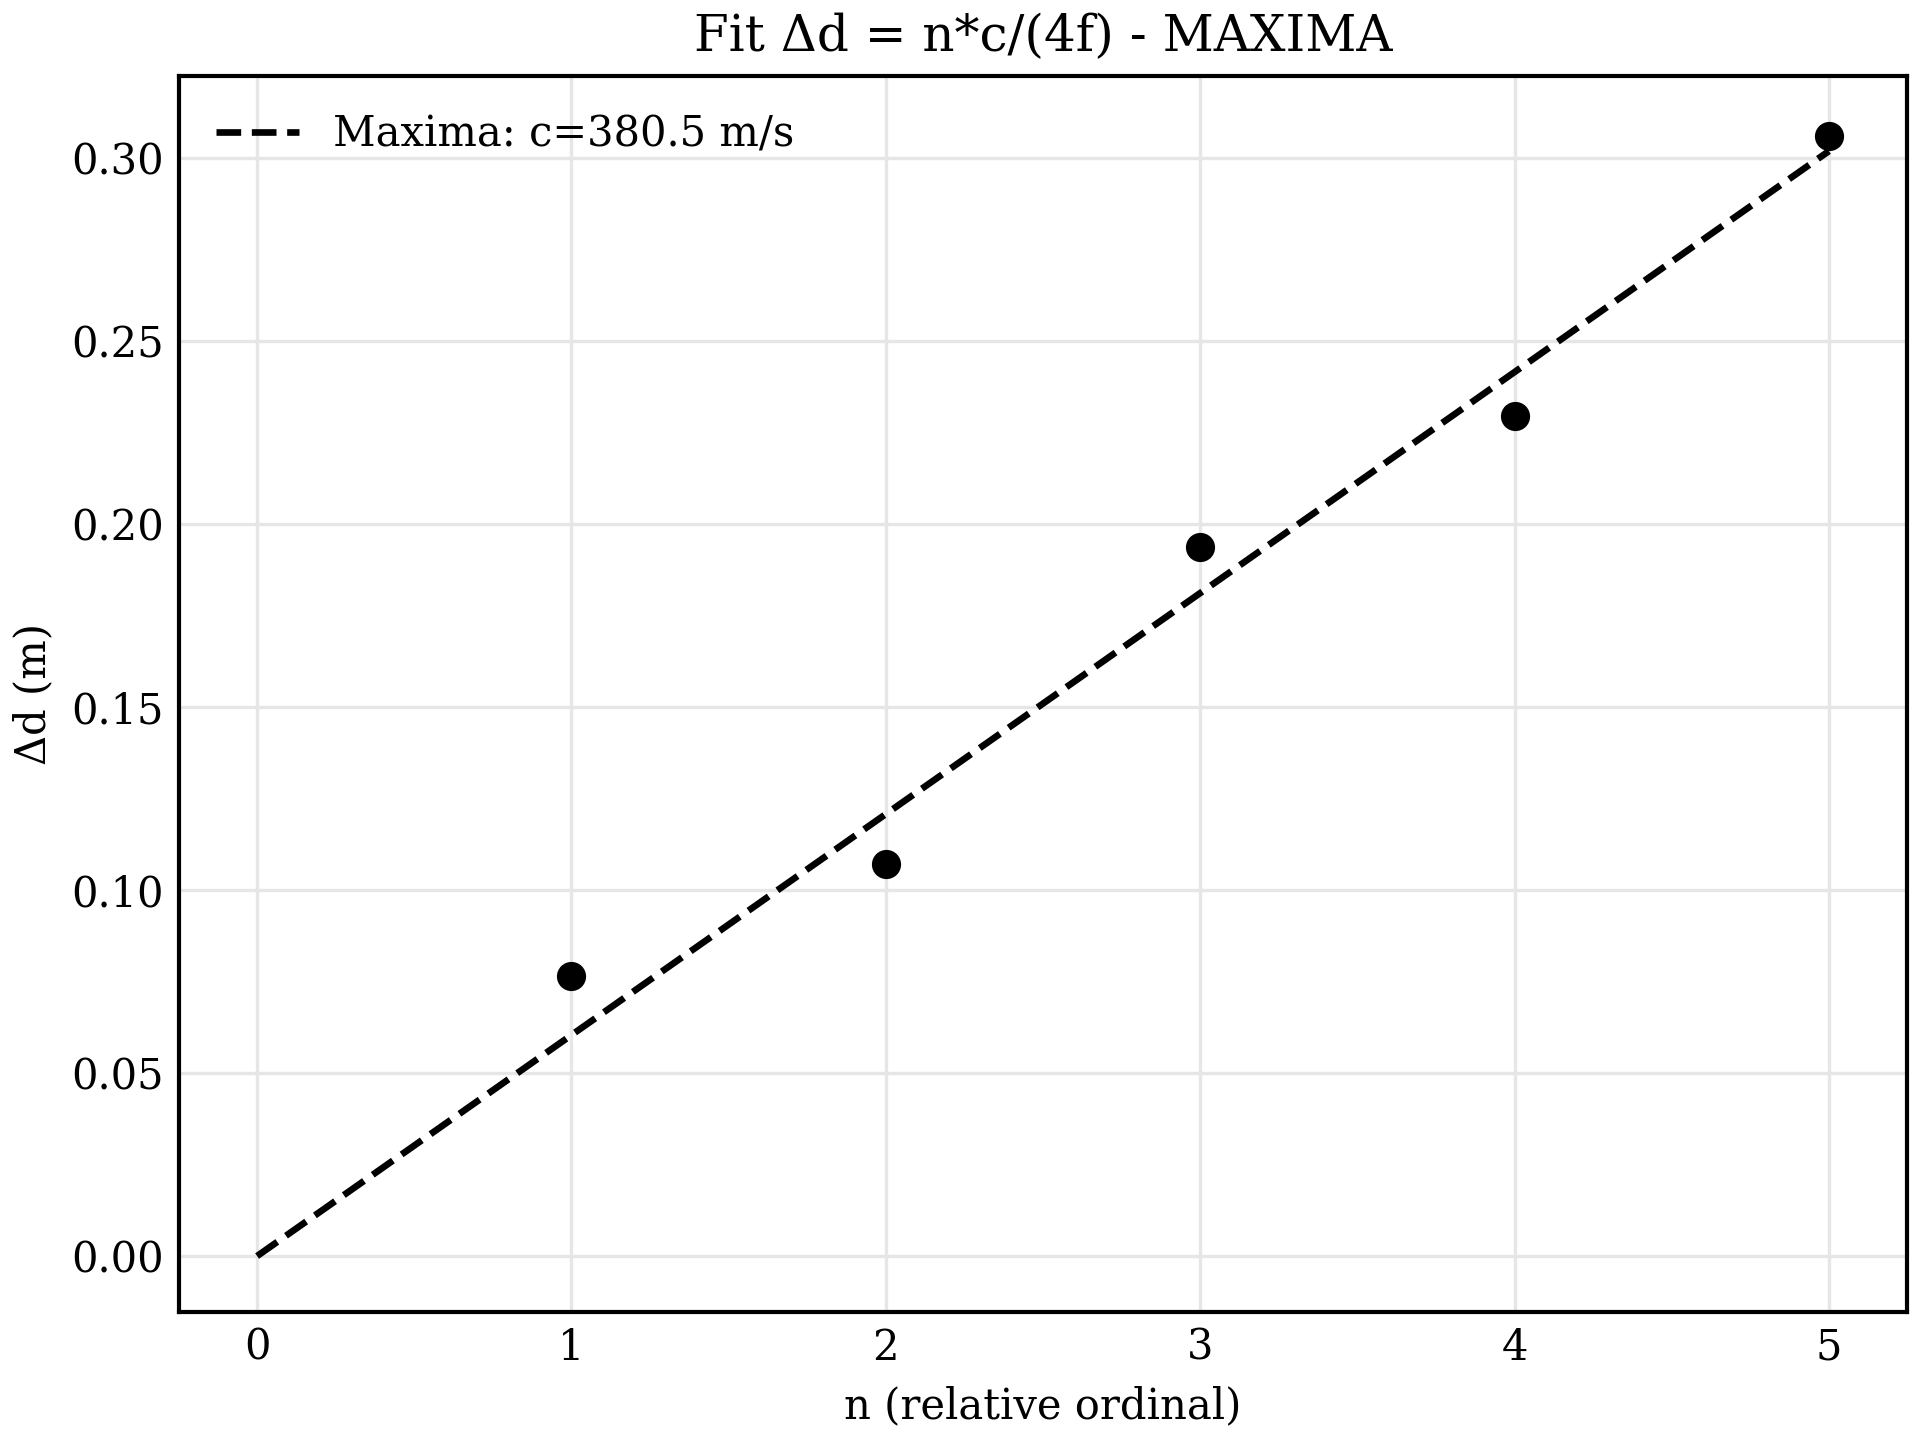
\includegraphics[width=0.45\textwidth]{m33_ajuste_maximos.png}
    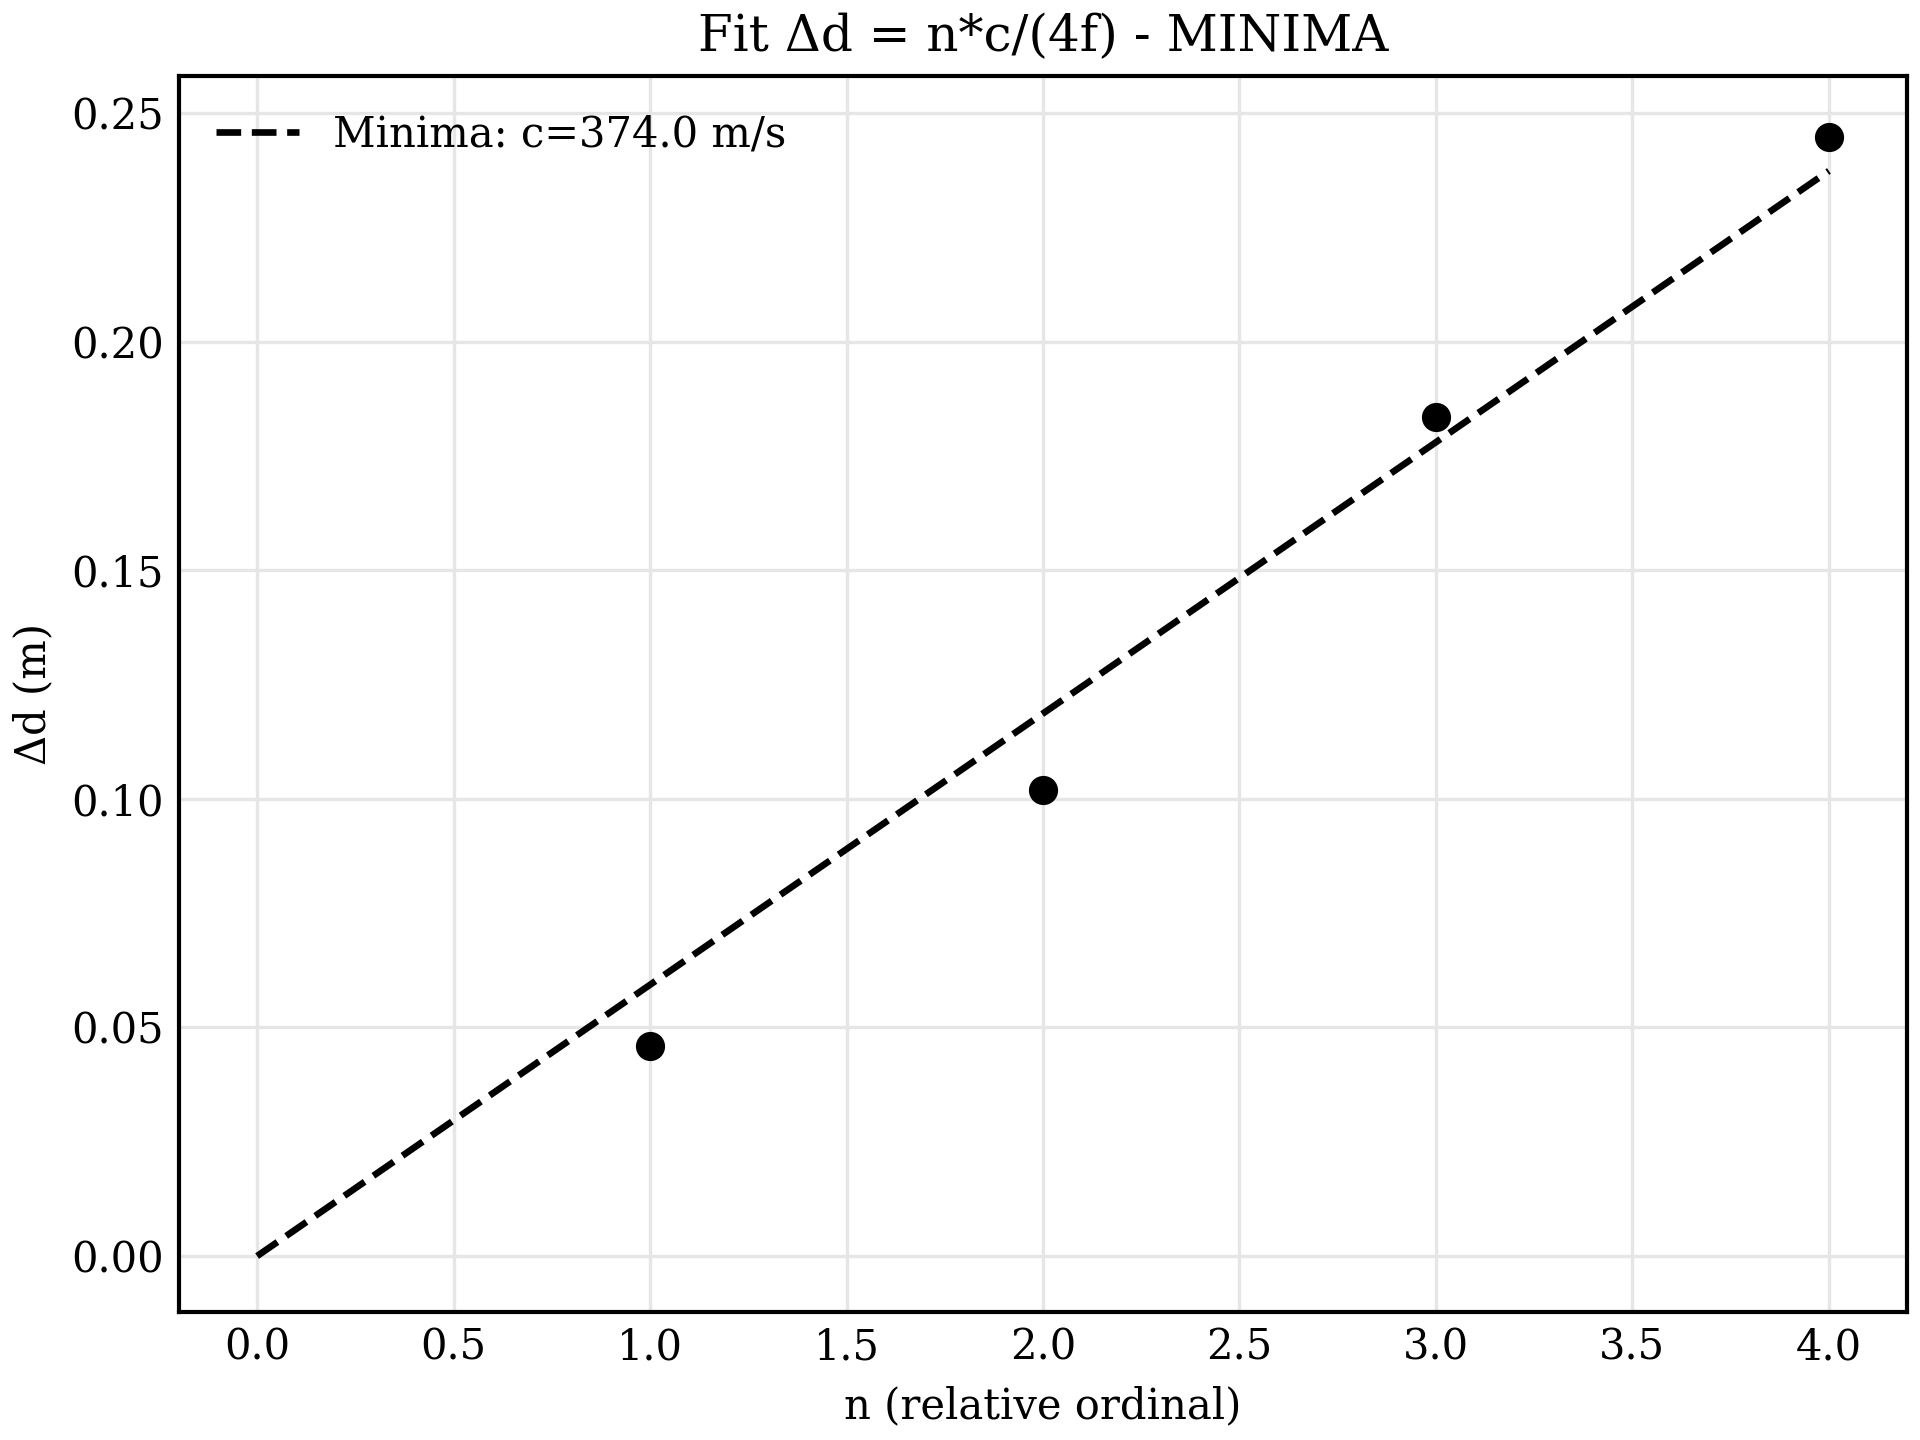
\includegraphics[width=0.45\textwidth]{m33_ajuste_minimos.png}
    \caption{Linear fits for sound speed determination using maxima (left) and minima (right).}
    \label{fig:fits}
\end{figure}

The resulting values for the speed of sound are:
\begin{itemize}
<<<<<<< HEAD
    \item \textbf{From Maxima}: $c = 380.54 \pm 0.85\,\mathrm{m/s}$
    \item \textbf{From Minima}: $c = 374.02 \pm 1.20\,\mathrm{m/s}$
\end{itemize}

The theoretical speed of sound at $\theta = 27.5\,^{\circ}\mathrm{C}$ (equivalent to $T = 300.65\,\mathrm{K}$) is calculated as:
\begin{equation}
    c_{theory} = 331.3 \sqrt{1 + \frac{\theta}{273.15}} = 331.3 \sqrt{\frac{300.65}{273.15}} = 347.58\pm0.29,\mathrm{m/s}
=======
    \item \textbf{From Maxima}: $c = \qty{380.54 \pm 0.85}{\unit{m/s}}$
    \item \textbf{From Minima}: $c = \qty{374.02 \pm 1.2}{\unit{m/s}}$
\end{itemize}

The theoretical speed of sound at $\theta = \qty{27.5}{^\circ C}$ (equivalent to $T = \qty{300.65}{K}$) is calculated as:
\begin{equation}
    c_{theory} = 331.3 \sqrt{1 + \frac{\theta}{273.15}} = 331.3 \sqrt{\frac{300.65}{273.15}} = \qty{347.58}{\unit{m/s}}
>>>>>>> c4b7d17 (supercipotes)
\end{equation}

The relative differences between the experimental and theoretical values are:
\begin{itemize}
    \item \textbf{Maxima}: 9.48 \%
    \item \textbf{Minima}: 7.61 \%
\end{itemize}

<<<<<<< HEAD
\subsection{Determination of the Characteristic Length ($a$)}
According to the theoretical model for a closed tube (Equation 3), the resonance frequencies $f_n$ are linearly dependent on the mode order $n$:
\begin{equation}
    f_n = n\frac{c}{2a}
\end{equation}

For a closed loop configuration, the allowed modes are even numbers ($n = 2, 4, 6\dots$). Therefore, the theoretical frequency difference between consecutive allowed modes ($\Delta n = 2$) is:
\begin{equation}
    \Delta f = 2 \frac{c}{2a} = \frac{c}{a}
\end{equation}

Based on the experimental data from Experiment A, four prominent resonance maxima were identified: $1380\,\mathrm{Hz}$, $1576\,\mathrm{Hz}$, $1660\,\mathrm{Hz}$, and $2070\,\mathrm{Hz}$. Assigning them a relative ordinal number $k = 1, 2, 3, 4$, a linear fit was performed to find the average frequency step between consecutive peaks.

The linear regression yields a slope of $m = 215.4\,\mathrm{Hz}$. The goodness of fit is characterized by a coefficient of Pearson $R^2 = 0.917$ and a reduced chi-squared $\chi^2_{red} = 1.41$.

\begin{figure}[H]
     \centering
     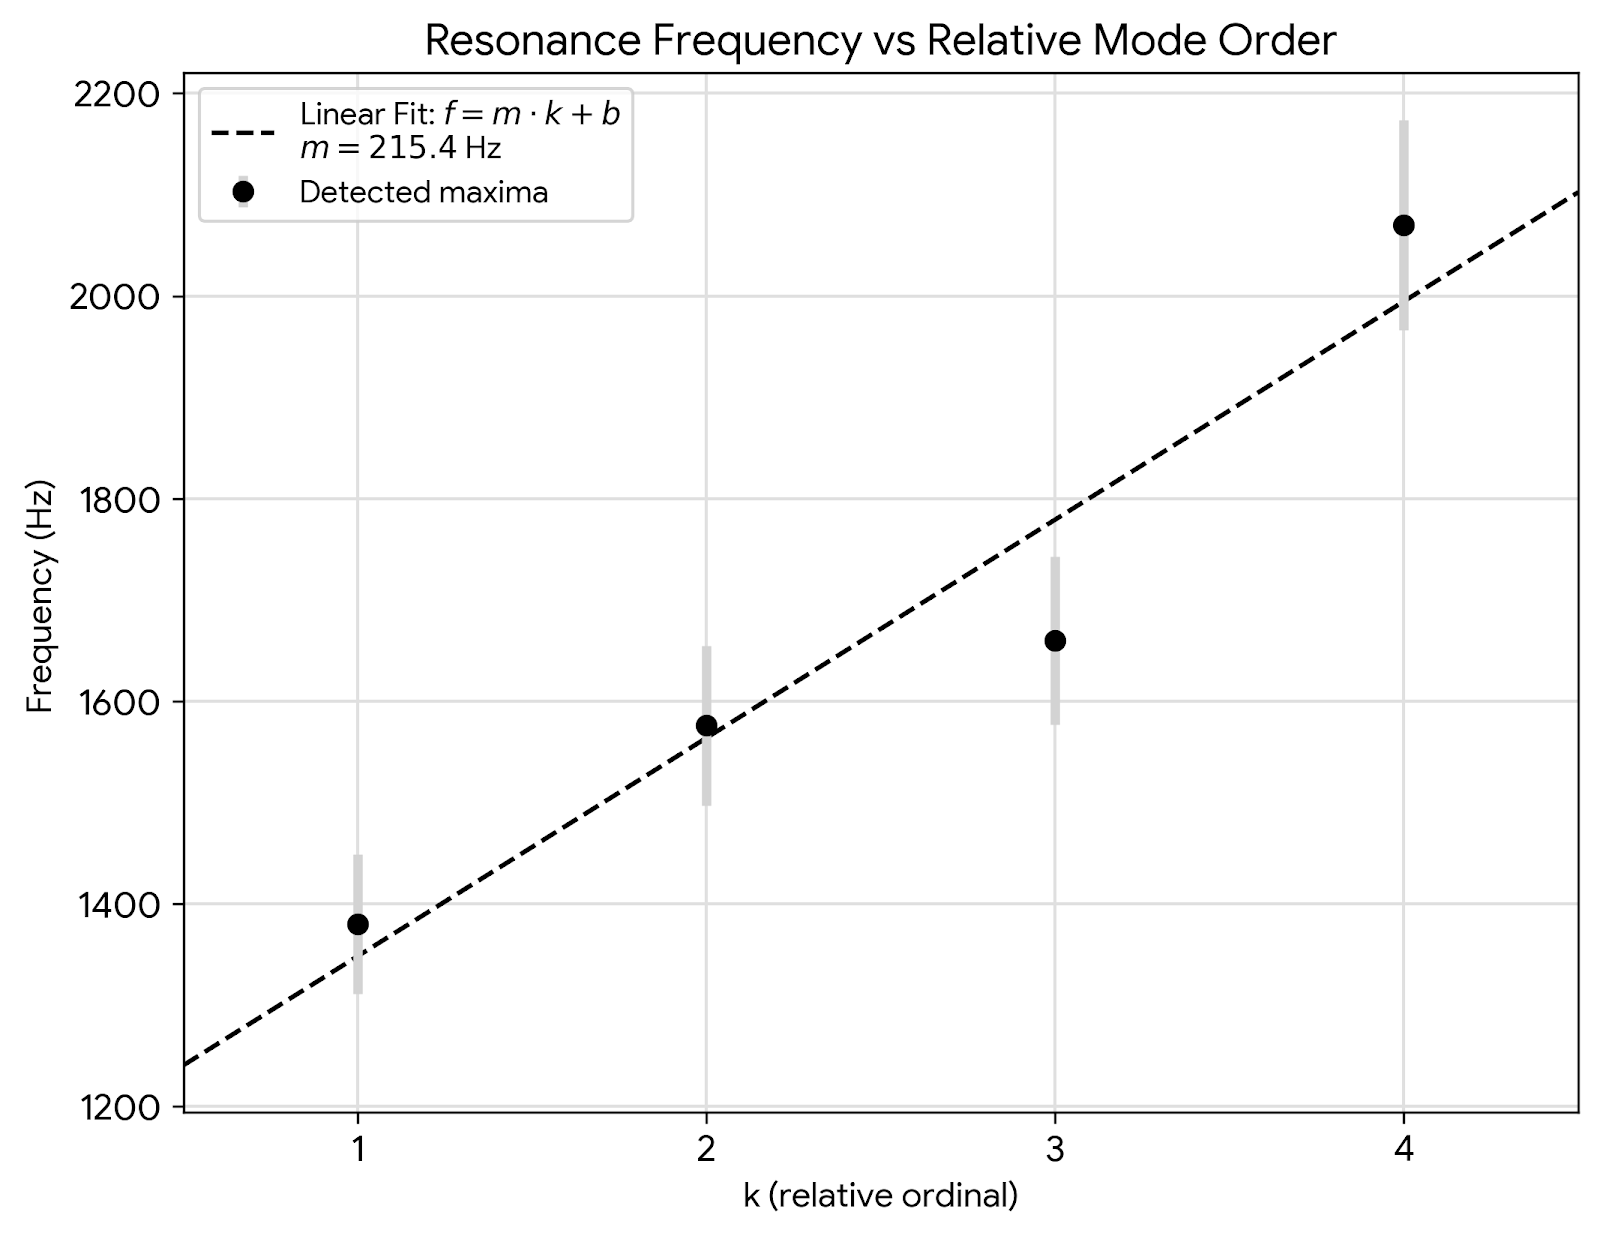
\includegraphics[width=0.6\textwidth]{unnamed.png}
     \caption{Resonance frequency as a function of relative mode order $k$.}
     \label{fig:freq_vs_k}
 \end{figure}

Using the experimental speed of sound obtained from the maxima fit ($c = 380.54\,\mathrm{m/s}$), the experimental value for the characteristic length of the Quincke tube is calculated as:
\begin{equation}
    a = \frac{c}{m} = \frac{380.54}{215.4} = 1.77\pm0.38,\mathrm{m}
\end{equation}


\section{Discussion and Conclusions}
In this experiment, the phenomena of constructive and destructive interference of acoustic waves were observed using a Quincke tube.

The speed of sound was determined experimentally using: the positions of the interference maxima and the interference minima. The linear fits yielded $c = 380.54 \pm 0.85\,\mathrm{m/s}$ (from maxima) and $c = 374.02 \pm 1.20\,\mathrm{m/s}$ (from minima). Both values are higher than the theoretical speed of sound at the laboratory temperature of $27.5\,^{\circ}\mathrm{C}$, which was calculated to be $347.58\,\mathrm{m/s}$. The relative errors were 9.48\% and 7.61\%, respectively.

Even though the order of magnitude is correct, the deviation suggests the presence of some errors in the setup. These differences could be due to these factors:
\begin{itemize}
    \item The theoretical calculation assumes a constant temperature inside the tube for the entire experiment. However, the electronical devices could have warmed the air, which would increase the actual speed of sound, or just the laboratorytemperature changed, as it was measured only at the beginning of the expiremnet.
    \item The scale on the movable arm might not be perfect and adjusting it by hand introduces some mechanical error.
    \item The formulas used in order to obatian the results assume perfect plane waves. The real world conditions make the waves behave slightly differently.
\end{itemize}

Finally, fitting all the resonance peaks together gives us a characteristic length of $a = \ensuremath{1.77 \pm 0.38\,\mathrm{m}}$. This result is probably really big compared to the actual size of the physical tube in the laboratory. The quality of this linear fit is also reflected by $\chi^2_{red} = 1.41$, which show that the data points do not follow a single straight line as the ideal model assumes.

This result might mean that some of the measured frequencies may not be resonances of the tube. This can explain the error and the reault of the $\chi^2_{red}$ obtained which is higher than 1. This can be due to some mistakes at the time of measuring the frequencies of the peaks, or just because some of the peaks are not peaks and have just been mistaken for peaks.

If we eliminate the two middle peaks and only use the \qty{1380}{Hz} and \qty{2070}{Hz} peaks which if we observe well, they are the theoretical $n=4$ and $n=6$ modes, as if we divide them by the n values both of them gives us exactly 345, the calculated length would be $a \approx \qty{0.55}{m}$. This value is much more realistic for the laboratory equipment.

\appendix
\section{Uncertainty Analysis}

\subsection{Direct Measurements and Instrumental Errors}
The uncertainties associated with the laboratory equipment were established as follows:
\begin{itemize}
    \item \textbf{Acoustic Amplitude (Voltage, $V$):} The digital oscilloscope and voltmeter system introduces a combined scale and reading uncertainty specified as:
    \begin{equation}
        u_V = 0.05 \cdot V + 0.001\,\mathrm{V}
    \end{equation}
    \item \textbf{Source Frequency ($f$):} The digital function generator presents a conservative structural tolerance of $5\%$ of the selected nominal value:
    \begin{equation}
        u_f = 0.05 \cdot f
    \end{equation}
    \item \textbf{Movable Arm Displacement ($\Delta d$):} The metric scale engraved on the physical tube allows a reading precision limited by its minor division and parallax effects, set as:
    \begin{equation}
        u_{\Delta d} = 0.001\,\mathrm{m} \quad (0.1\,\mathrm{cm})
    \end{equation}
    \item \textbf{Laboratory Ambient Temperature ($\theta$):} Measured with a standard wall thermometer with an absolute resolution of:
    \begin{equation}
        u_\theta = 0.5\,^{\circ}\mathrm{C}
    \end{equation}
\end{itemize}

\subsection{Propagation in Theoretical Speed of Sound}
The theoretical speed of sound depends exclusively on the ambient temperature according to the expression $c_{theory}(\theta) = 331.3 \sqrt{1 + \theta/273.15}$. Applying the first-order Taylor series expansion for non-correlated variables, the propagated uncertainty $u_{c_{theory}}$ is derived via the partial derivative with respect to $\theta$:
\begin{equation}
    u_{c_{theory}} = \left| \frac{\partial c_{theory}}{\partial \theta} \right| u_\theta = \frac{331.3}{2 \cdot 273.15 \cdot \sqrt{1 + \frac{\theta}{273.15}}} u_\theta
\end{equation}

Substituting $\theta = 27.5\,^{\circ}\mathrm{C}$ and $u_\theta = 0.5\,^{\circ}\mathrm{C}$:
\begin{equation}
    u_{c_{theory}} = \frac{331.3}{546.3 \cdot 1.049} \cdot 0.5 = 0.29\,\mathrm{m/s}
\end{equation}
Yielding a theoretical reference value of $c_{theory} = 347.58 \pm 0.29\,\mathrm{m/s}$.

\subsection{Propagation in Characteristic Length ($a$)}
The experimental determination of the characteristic length of the tube arm is governed by the functional dependence $a(c, m) = \frac{c}{m}$, where $c$ is the sound velocity obtained from the interference maxima and $m$ is the slope of the resonance frequency fit. 

Assuming $c$ and $m$ are independent parameters, the absolute uncertainty $u_a$ is calculated using the variance formula:
\begin{equation}
    u_a = \sqrt{\left( \frac{\partial a}{\partial c} \right)^2 u_c^2 + \left( \frac{\partial a}{\partial m} \right)^2 u_m^2} = \sqrt{\left( \frac{1}{m} \right)^2 u_c^2 + \left( - \frac{c}{m^2} \right)^2 u_m^2}
\end{equation}

This expression can be rewritten compactly in terms of quadrature relative errors:
\begin{equation}
    u_a = a \sqrt{\left( \frac{u_c}{c} \right)^2 + \left( \frac{u_m}{m} \right)^2}
\end{equation}

Introducing the experimental variables extracted from the analysis of all identified peaks:
\begin{itemize}
    \item Speed of sound from maxima fit: $c = 380.54 \pm 0.85\,\mathrm{m/s}$
    \item Slope from relative mode fit: $m = 215.4 \pm 45.9\,\mathrm{Hz}$
    \item Nominal length value: $a = 1.767\,\mathrm{m}$
\end{itemize}

Evaluating the numerical propagation:
\begin{equation}
    u_a = 1.767 \sqrt{\left( \frac{0.85}{380.54} \right)^2 + \left( \frac{45.9}{215.4} \right)^2} = 1.767 \sqrt{4.99\times 10^{-6} + 0.0454} = 0.377\,\mathrm{m}
\end{equation}

Rounding to two significant figures for the uncertainty and matching the decimal precision in the nominal value, the final experimental parameter is reported as:
\begin{equation}
    a = 1.77 \pm 0.38\,\mathrm{m}
\end{equation}
=======
\section{Discussion and Conclusions}
% [HUMAN AUTHOR: WRITE DISCUSSION/CONCLUSIONS HERE]

\appendix
\section{Uncertainty Analysis}
The uncertainty in voltage $u_V$ was calculated as $5\%$ of the reading plus an instrumental offset of $0.001 \unit{V}$. The uncertainty in frequency $u_f$ was estimated as $5\%$ of the set value. For the distance $\Delta d$, a fixed uncertainty of $0.1 \unit{cm}$ was assumed based on the scale of the movable arm. The uncertainty in the fitted speed of sound was derived from the variance of the weighted linear fit through the origin.
>>>>>>> c4b7d17 (supercipotes)

\end{document}